
\chapter[Breaking isometric ties and introducing priors in Gromov-Wasserstein distance]{Breaking isometric ties and introducing priors in Gromov-Wasserstein distance}
\label{chap:agw}

\renewcommand{\contentsname}{Contents}
\localtableofcontents*
\chaptermark{\textbf{Breaking isometric ties and introducing priors in Gromov-Wasserstein distance}}

\hfill \break
This section presents the results from \citep{Demetci23} and address the problem of
incorporating priors into Gromov-Wasserstein distance.
Gromov-Wasserstein distance has many applications in machine learning due to its ability
to compare measures across metric spaces and its invariance to isometric transformations. However,
in certain applications, this invariant property can be too flexible, thus undesirable. Moreover,
the Gromov-Wasserstein distance solely considers pairwise sample similarities in input datasets,
disregarding the raw feature representations. We propose a new optimal transport formulation,
called Augmented Gromov-Wasserstein (AGW), that allows for some control over the
level of rigidity to transformations. It also incorporates feature alignments,
enabling us to better leverage prior knowledge on the input data for improved performance.
We present theoretical insights into the proposed method. We then demonstrate its usefulness
for single-cell multi-omic alignment tasks and heterogeneous domain adaptation in machine learning.

% \paragraph{Contributions} PD, IR and RS designed and planned the study. All authors wrote
% the paper and revised the manuscript. by PD and RS did the experimental design and analysis.
% The theoritical analysis of the proposed method is performed by QHT and revised by IR.

\raggedbottom

%%%%%%%%%%%%%%%%%%%%%%%%%
\section{Introduction}

Optimal transport (OT) theory provides a fundamental tool for comparing and
aligning probability measures omnipresent in machine learning (ML) tasks.
Following the least effort principle, OT and its associated metrics offer
many attractive properties that other divergences, such as the popular Kullback-Leibler or
Jensen-Shannon divergences, lack. For instance, OT borrows key geometric properties of
the underlying ``ground'' space on which the distributions are defined \citep{Villani03}
and enjoys non-vanishing gradients when measures have disjoint support \citep{Arjovsky17}.
OT theory has also been extended to a much more challenging case of probability measures supported
on different metric-measure spaces. In this scenario, the Gromov-Wasserstein (GW) distance
seeks an optimal matching between points in the supports of the considered distributions
that will minimize the distortion of intra-domain distances upon such matching.

Since its proposal by \citet{Memoli11} and further extensions by \citet{Peyre16},
GW has been successfully used in a wide range of applications, including
domain adaptation \citep{Yan18}, computational biology
\citep{Nitzan2019,Pamona,UniPort,SpaOTsc,Demetci20,Demetci22,PASTE},
generative modeling \citep{Bunne19}, and reinforcement learning \citep{GW-VAE}.

\paragraph{Limitations of prior work} Successful applications of GW distance are often
attributed to its invariance to distance-preserving transformations (also called ``isometries'')
of the input domains. Since GW considers only intra-domain distances, it is naturally invariant
to any transformation that does not alter them. While this is a blessing in many applications,
for example, comparing graphs with the unknown ordering of nodes, it may become a curse
when one has to choose the ``right'' isometry among many that yield the same GW distance.
How could one break such ties while keeping the attractive properties of the GW distance?
This question remains to be addressed in the field.

Additionally, GW distances are often used in tasks where one may have some
\textit{a priori} knowledge about the mapping between the two considered spaces.
For example, in single-cell applications, mapping a group of cells in similar tissues
across species helps understand the evolutionarily conserved and diverging cell types
and functions \citep{kriebel2022uinmf}. When performed using OT, this cross-species cell mapping
may benefit from the knowledge about an overlapping set of orthologous genes
\footnote {Genes in two different species that originated from a common ancestor and
largely maintained their function and sequence during speciation}.
GW formulation does not offer any straightforward way to incorporate this knowledge,
which may lead to suboptimal performance.

\paragraph{Our contributions}
In this chapter, we introduce a new OT formulation that addresses the drawbacks of the
GW distance mentioned above. We summarize our contributions as follows:
\begin{enumerate}
    \item We propose Augmented Gromov-Wasserstein (AGW), a new formulation that leverages
    both pairwise sample similarities in input datasets and their raw data representations;
    \item We demonstrate that AGW allows for better control over the isometric transformations
    of the GW distance and helps break isometric ties;
    \item We show that AGW can incorporate prior knowledge to guide how the two metric spaces
    should be compared, which improves object comparisons; %object matchings; Priors can also be set to further tighten isometric invariances
    \item We provide a theoretical analysis of the properties of the proposed formulation
    and examples that concretely illustrate its unique features;
    \item Our empirical results show that AGW outperforms previously proposed
    cross-domain OT methods in several downstream tasks and tends to converge in fewer iterations
    than GW. We first focus on real-world applications in computational biology,
    namely the single-cell data integration tasks. Then, we also illustrate its generalizability
    to the heterogeneous domain adaptation in ML.
    %\item runtime
\end{enumerate}
% The paper is organized as follows. Section 2 presents key notions from the OT theory
% utilized in the rest of the paper. Section 3 presents our proposed AGW formulation and
% analyzes its theoretical properties. In Section 4, we present several empirical studies
% for the single-cell alignment task and demonstrate the applicability of our method to
% the heterogeneous domain adaptation task. We conclude our paper in Section 5 with
% a discussion of potential future work.

% \paragraph{Notations} In what follows, we denote by
% $\Sigma_{n}=\{ p \in \bbR_{> 0}^n: \sum_{i=1}^{n} p_{i}=1\}$
% the simplex histogram with $n$ bins. We use $\otimes$ for tensor-matrix multiplication,
% \ie, $L \otimes B$ is the matrix $(\sum_{k,l} L_{ijkl} B_{kl})_{i,j}$ for a $4$D-tensor $L$ and
% a matrix $B$. We use $\langle \cdot, \cdot \rangle$ for the matrix scalar product associated with
% the Frobenius norm $\|\cdot\|_{F}$. We write $1_d \in \bbR^d$ for a
% $d$-dimensional vector of ones. We use the terms ``coupling matrix'', ``transport plan''
% and ``correspondence matrix'' interchangeably.
% A point in the space can also be called ``an example'' or ``a sample''.
% Given an integer $n \geq 1$, denote $[n] := \{ 1, ..., n\}$.

%%%%%%%%%%%%%%%%%%%%%%%%%%%%%%%%%%%%%%%%%%%%%%%
\section{Augmented Gromov-Wasserstein}

\begin{figure}[t]
\centering
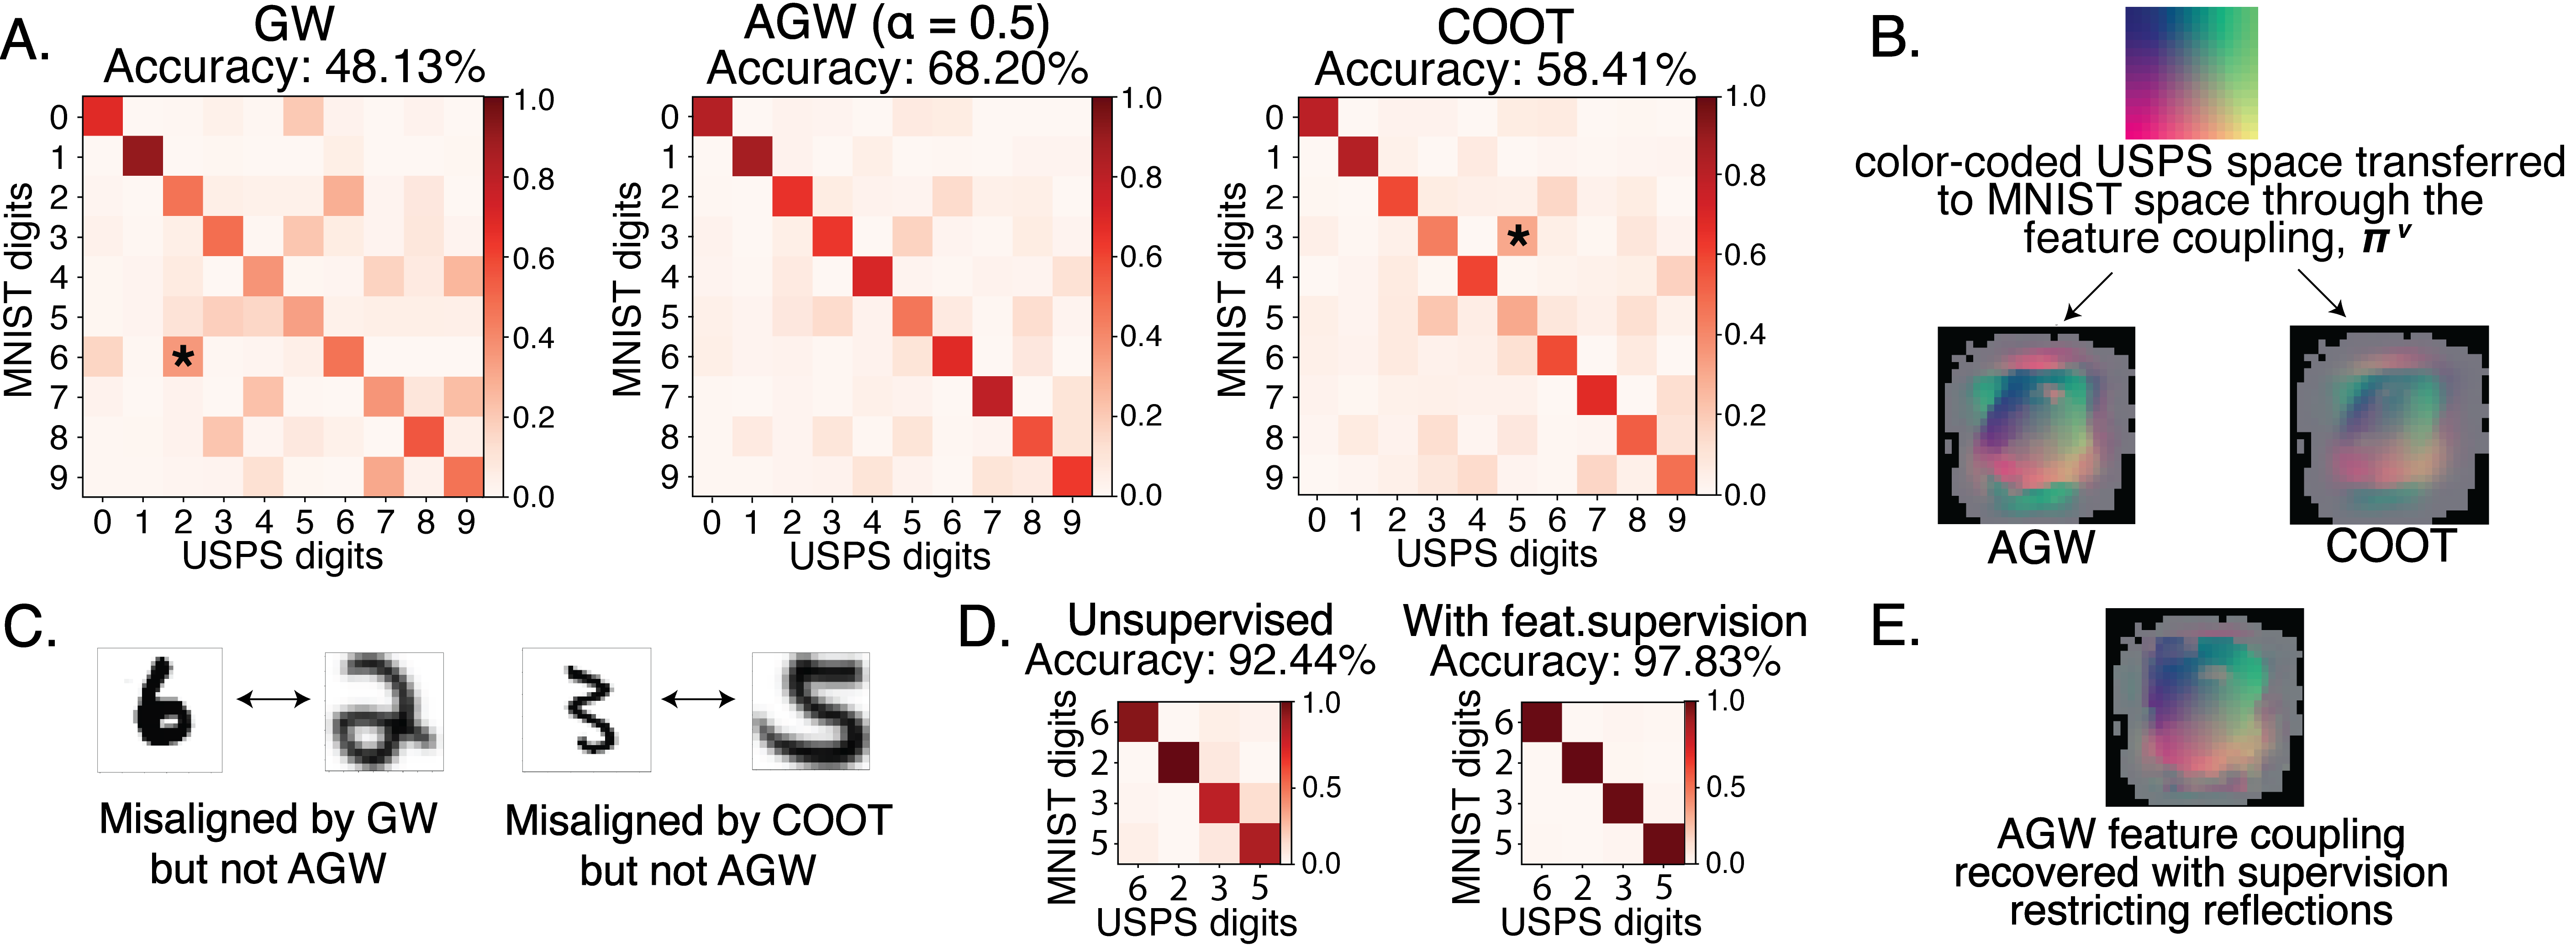
\includegraphics[width=\linewidth]{./Chapitre5/fig//mnist1_supervised.png}
\caption{Aligning digits from MNIST and USPS datasets. \textbf{(A)}
Confusion matrices of GW, AGW with $\alpha=0.5$ and COOT.
(*) denote pair alignments ;
\textbf{(B)} Feature coupling $Q$ of AGW compared to COOT;
\textbf{(C)} Illustration of a case from where GW's and COOT's invariants are
detrimental for obtaining a meaningful comparison, while AGW remains informative.
\textbf{(D)} Example showing improved digit alignment with feature-level supervision
that restricts reflections \textbf{(E)} Feature coupling recovered by AGW ($\alpha =0.5$)
in the supervised setting of (D).}
\label{fig:mnist}
\end{figure}

Here, we start by outlining the motivation for our proposed formulation,
highlighting the different properties of GW distance and COOT. Then,
we detail our AGW method that interpolates between the two, followed by a
theoretical study of its properties.

\subsection{Motivation}

\paragraph{Invariants of GW} GW distance remains unchanged under isometric transformations of
the input data. This property has contributed much to the popularity of GW distance,
as isometries naturally appear in many applications. However,
not all isometries are equally desirable. For instance, a rotation of the
handwritten digit $6$ seen as a discrete measure can lead to its slight variation
for small angles or to a digit $9$ when the angle is close to $180$ degrees. In both cases,
however, the GW distance remains unchanged, making it insufficient to distinguish
the two digits apart.

\paragraph{Invariants of COOT} Unlike GW, COOT has fewer degrees of freedom
in terms of invariance to global isometric transformations as it is limited to
permutations of rows and columns of the two matrices, and not all isometric transformations
can be achieved via such permutations.

Additionally, COOT is strictly positive for any two datasets of different sizes either
in terms of features or samples, making it much more restrictive than GW.
It thus provides a fine-grained control when comparing complex objects,
yet it lacks the robustness of GW to frequently encountered transformations
between the two datasets. Further, unlike GW, it is invariant to local isometries
that can be achieved via permutations of a subset of features.

\subsection{AGW formulation} \label{subsec:agw_formulation}
Given the above discussion on the invariants of COOT and GW distance,
interpolating between them will restrict each other's invariants. Additionally,
interpolating with COOT is a natural way to introduce raw feature alignments in GW,
which allows for leveraging priors on them. We call this interpolation \textbf{Augmented GW} (AGW).
Recall that a weighted matrix is the triplet $\cX = (X, \mu_1^X, \mu_2^X)$, where
$X \in \bbR^{n_x \times d_x}, \mu_1^X \in \Delta_{n_x}$ and $\mu_2^X \in \Delta_{d_x}$.
Given $\alpha \in [0,1]$, we define the AGW between two weighted matrices $\cX$ and $\cY$ as
\begin{align}
\label{eq:scootr}
\agw_{\alpha}(\cX, \cY) &:=
\min_{\substack{P \in U(\mu_1^X, \mu_1^Y) \\ Q \in U(\mu_2^X,\mu_2^Y)}} \quad
\alpha \; \langle L(C^x,C^y) \otimes P, P \rangle + (1-\alpha) \; \langle L(X,Y) \otimes P, Q \rangle,
\end{align}
where
\begin{itemize}
    \item[$\bullet$] $\langle L(C^x,C^y) \otimes P, P \rangle
    = \sum_{i,j,k,l} \; (C^x_{ik} - C^y_{jl})^2 P_{ij} P_{kl}$ is the objective function of
    the GW distance. Here, the matrices $C^x \in \bbR^{n_x \times n_x}$ and
    $C^y \in \bbR^{n_y \times n_y}$
    contain the intra-domain pairwise distances between the rows of $X$ and $Y$, respectively.

    \item[$\bullet$] $\langle L(X,Y) \otimes P, Q \rangle =
    \sum_{i,j,k,l} \; (X_{ik} - Y_{jl})^2 P_{ij} Q_{kl}$ is the objective function of the COOT.
\end{itemize}
The AGW problem always admits a solution. Indeed, as the objective function is continuous
and the sets of admissible couplings are compact, the existence of minimum and minimizer
is guaranteed.

When $\alpha = 1$, we recover the GW distance, whereas $\alpha = 0$ corresponds to the
COOT. Our interpolation offers several important benefits. First, COOT term ensures that AGW
will take different values for any two isometries whenever $d_x \neq d_y$. Intuitively,
AGW's value will then depend on how ``far'' a given isometry is from a permutation of rows
and columns of the inputs. Thus, we restrict a broad class of (infinitely many) transformations
that GW cannot distinguish and we tell them apart by assessing whether they
can be approximately obtained by simply swapping 1D elements in input matrices.

Second, combining the objective functions of COOT and GW distance allows us to
effectively influence the optimization of $P$ by introducing priors on feature matchings
through $Q$ and vice versa. This can be achieved by penalizing the costs of matching
certain features in the COOT term to influence the optimization of $Q$. This prior knowledge
guides how the two metric spaces should be compared and improves empirical performance.
These key properties explain our choice of calling it ``augmented'':
we equip GW distance with an ability to provide finer-grained object comparisons by
breaking isometric ties and/or guiding the matching using available prior knowledge.

\paragraph{Illustrations} We illustrate AGW's properties on a task of aligning handwritten digits
from MNIST \citep{lecun10} (28$\times$28 pixels) and USPS datasets (16$\times$16 pixels)
\citep{Hull94} in \Cref{fig:mnist}, where AGW with $\alpha=0.5$ outperforms both GW and COOT
in alignment accuracy (Panel A). The black asterisks show the digit pairs that most benefit
from AGW interpolation, which are $6-2$ for GW and $3-5$ for COOT.
Panel C visualizes examples from these digit pairs that are misaligned by GW and COOT
but not by AGW.
\footnote{Here, we define ``aligned pairs'' as pairs of digits with the
highest coupling probabilities.}. Here, we observe that 6-2 misalignment by GW is likely because
one is a close reflection of the other across the y-axis. Similarly,
COOT mismatches 3 and 5 as one can obtain 3 from 5 by a local permutation of
the upper half of the pixels. Panel B visualizes the feature couplings obtained by
AGW (on the left) and COOT (on the right). The feature coupling by COOT confirms that
COOT allows for a reflection across the y-axis on the upper half of the image
but not on the lower half. With AGW, both of these misalignments improve,
likely because (1) the correct feature alignments in the lower half of the images
prevent 6 and 2 from being matched and (2) GW distance is non-zero for 5-3 matches
since the transformation is not applied to the whole image. In Panels D and E,
we also show that providing supervision on feature alignments to restrict local reflections
further improves AGW's performance.

Similar improvement can be seen for aligning cells (samples) for two different single-cell
measurements (features) \citep{SNAREseq} in Figure S2. Panel A shows that AGW consistently maps
the 4 cell types in the data better than GW (a popular method for this task
\citep{Pamona,Demetci20,Demetci22,UniPort}) over 50 random subsampling of cells.
The 2D projection of alignments in Panel B shows that GW sometimes completely swaps
the cell type clusters when they have a similar number of cells, whereas AGW is more robust
to this phenomenon.

\paragraph{Optimization} For simplicity, suppose $n_x = n_y = n$ and $d_x = d_y = d$.
With the squared loss in both GW and COOT terms, the computational trick by \citet{Peyre16}
can be applied, which reduces the complexity of AGW from $O(n^4 + n^2 d^2)$
to $O(n^3 + dn^2 + nd^2)$. For optimization, we use the block coordinate descent (BCD) algorithm,
where we alternatively fix one coupling and minimize AGW with respect to the other (\Cref{alg:bcd_agw}).
Each iteration then consists of solving two OT problems. To further accelerate the optimization,
entropic regularization can be used \citep{Cuturi13} on either $P$, $Q$, or both.
In practice, we rely on the built-in functions of the Python Optimal Transport package \citep{Flamary21}.

\begin{algorithm}[t]
    \caption{BCD algorithm to solve AGW \label{alg:bcd_agw}}
    \begin{algorithmic}[1]
      \STATE Initialize $P^*$ and $Q^*$.
      \REPEAT
      \STATE Calculate $L_Q = L(X, Y) \otimes P^*$.
      \STATE For fixed $P$, solve the OT problem:
      $Q^* \in \argmin_{Q \in U(\mu_2^X, \mu_2^Y)} \langle L_Q, Q \rangle$.
      \STATE Calculate $L_P = L(X, Y) \otimes Q^*$.
      \STATE For fixed $Q$, solve the fused GW problem:
      \begin{align}
        P^* \in \argmin_{P \in U(\mu_1^X, \mu_1^Y)}
        \alpha \; \langle L(D_X,D_Y) \otimes P, P \rangle + (1-\alpha) \langle L_P, P \rangle.
      \end{align}
      \UNTIL{convergence}
\end{algorithmic}
\end{algorithm}

%%%%%%%%%%%%%%%%%%%%%%%%%%%%%%%%%%%%%%%%%%%%%%
\subsection{Theoretical analysis} \label{subsec:agw_property}

\paragraph{Preliminary results}
Intuitively, we expect that AGW interpolates between GW and COOT and shares similar properties
with Fused Gromov-Wasserstein (FGW) distance \citep{Vayer19b}, namely
the relaxed triangle inequality (since COOT and GW distances are both metrics).
The following result summarizes these observations, whose proofs are presented in
Appendix \ref{appendix:agw}.
\begin{proposition}
\label{prop:basic_prop}
For $\alpha \in [0, 1]$,
\begin{enumerate}
    \item Given two weighted matrices $\cX$ and $\cY$, when $\alpha \to 0$ (or $1$),
    one has $\agw_{\alpha}(\cX, \cY) \to \coot(\cX, \cY)$ (or $\gw(\cX, \cY)$).

    \item AGW satisfies the relaxed triangle inequality: for any weighted matrices $\cX, \cY$
    and $\cZ$, one has $\agw_{\alpha}(\cX, \cY) \leq 2 \big( \agw_{\alpha}(\cX, \cZ)
    + \agw_{\alpha}(\cZ,  \cY) \big)$.
\end{enumerate}
\end{proposition}

\paragraph{Invariants of AGW}
A more intriguing question is about the invariants that AGW exhibits.
We denote $\cO_d$ and $\cP_d$ the sets of orthogonal and permutation matrices of size $d$,
respectively. Given a matrix $X \in \bbR^{n \times d}$, we assume that
\begin{assumption}
    \label{assumption:1}
    $X$ is full-rank and has exactly $\min(n, d)$ distinct singular values.
\end{assumption}
The full-rank assumption is not uncommon in the machine learning literature \citep{Kenji19}
and can be easily met in practice. Additionally,
not only the Hermitian matrices with repeated eigenvalues are rare (see page 56 in \citep{Tao12}),
but we can even show that
\begin{corollary}
\label{corr:hermitian}
    The set of Hermitian matrices with repeated eigenvalues has zero Lebesgue measure.
\end{corollary}
Since the singular values of $X$ are determined by the symmetric matrix $X X^T$,
\Cref{corr:hermitian} assures that it is reasonable to exclude all symmetric matrices
with repeated eigenvalues. With these, we present:
\begin{theorem}
\label{thm:invariant}
Given two weighted matrices $\cX$ and $\cY$.
\begin{enumerate}
    \item If $\mu_1^X = \mu_1^Y$ and $Y$ is obtained by permuting columns of
    $X$ via the permutation $\sigma_c$ (so $\mu_2^Y = (\sigma_c)_{\#} \mu_2^X$),
    then $\agw_{\alpha}(\cX, \cY) = 0$.
    \item Suppose $X \in \bbR^{n \times d}$, where $n \geq d$, satisfies \Cref{assumption:1}.
    For any $0 < \alpha < 1$, if $\agw_{\alpha}(\cX, \cY) = 0$,
    then there exist a symmetric orthogonal matrix $O \in \cO_d$ and
    a permutation matrix $P \in \cP_d$ such that $Y = X OP$.
\end{enumerate}
\end{theorem}
Despite the simplicity of the interpolation structure, the invariants induced by AGW
present novel and non-trivial challenges for theoretical analysis.
While sharing basic invariants, such as feature swaps, AGW covers much fewer isometries than
GW distance. Similar to COOT, AGW only has at most finitely many, whereas GW has infinitely many isometries.
Under mild conditions, when AGW vanishes, only transformations with a particular structure
(compositions of a permutation and a symmetric orthogonal transformation) are eligible.
Given the superior empirical performance of AGW over GW and COOT, such isometries appear
meaningful and relevant in real-world tasks.

\paragraph{Weak invariant to translation}
While enjoying the interpolation and metric properties, AGW does not inherit the invariant
to the translation of the GW distance. However, we find that it satisfies a relaxed version
of this invariant defined as follows.
\begin{definition}
    We call $D = \inf_{\pi \in \cU} F(\pi, X, Y)$, where $X, Y$ are input data and $\cU$
    is a set of feasible couplings and $F$ is a real-valued functional, an OT-based divergence.
    Then $D$ is weakly invariant to translation if for every $a, b \in \bbR$, we have
    $\inf_{\pi \in U} F(\pi, X + a, Y+b) = \inf_{\pi \in \cU} F(\pi, X, Y) + c$,
    for some constant $C$ depending on $a, b, X, Y$ and $\cU$.
\end{definition}
Here, we denote the translation of $X$ as $X + a$, whose elements are of the form $X_{ij} + a$.
Intuitively, an OT-based divergence is weakly invariant to translation if only
the optimal transport plan is preserved under translation, but not necessarily the divergence itself.
In practice, we would argue that the ability to preserve the optimal plan under translation
is much more important than preserving the distance itself. In other words,
the translation only shifts the minimum but has no impact on the optimization procedure,
meaning that the minimizer remains unchanged. This is indeed the case of AGW.
\begin{proposition}
    \label{prop:invariant} For any $\alpha \in [0,1]$, AGW is weakly invariant to translation.
\end{proposition}

%%%%%%%%%%%%%%%%%%%%%%%%%%%%%ù
\subsection{Related work}

Most related to our work is the Fused Gromov-Wasserstein (FGW) distance \citep{Vayer19b}
that compares structured objects. Its objective function is a convex combination of
the GW term defined based on the pairwise intra-domain distances and the Wasserstein term
defined over additional features that live in the same space for both input matrices.
Despite the resemblance to FGW, AGW fundamentally differs from it in several ways.
Firstly, AGW uses explicit control over the invariants of GW to provide more meaningful
cross-domain matchings. No other OT-based metric in the literature (including FGW)
leverages a similar idea. As such, \Cref{thm:invariant} is the first result of its kind
aiming at characterizing the invariances resulting from such interpolation.

Secondly, FGW is mostly used for structured objects endowed with additional information living
in the same space, for example, two graphs where each node may be colored by
a specific color (``additional'' feature). On the other hand, AGW can be used on
empirical measures defined for any set of objects across domains, including ones
from different dimensional spaces, and requires no additional information.

Finally, the notion of feature space in FGW does not have the same meaning as in AGW.
The feature space in FGW is associated with the sample space, whereas in AGW (and also in COOT),
the two spaces are independent. Each element of the former is
associated with a point in the sample space. By contrast, the features in AGW are
precisely the coordinates of a point, in addition to its representation in the
original and dissimilarity-induced spaces.

%%%%%%%%%%%%%%%%%%%%%%%%%%%%%%%%%%%%%%%%
\section{Experimental evaluations}

\begin{table}[t]
\begin{center}
\resizebox{1.0\linewidth}{!}{
\begin{tabular}{lccccccc}
\hline
                                     & \textbf{Simulation 1}                                           & \textbf{Simulation 2}                                          & \textbf{Simulation 3}                                          & \textbf{Simulated RNA-seq}      & \textbf{scGEM}                                              & \textbf{SNARE-seq}                                                & \textbf{CITE-seq}                                             \\
                                     & \begin{tabular}[c]{@{}c@{}}(300x1000, \\ 300x2000)\end{tabular} & \begin{tabular}[c]{@{}c@{}}(300x1000,\\ 300x2000)\end{tabular} & \begin{tabular}[c]{@{}c@{}}(300x1000,\\ 300x2000)\end{tabular} & \begin{tabular}[c]{@{}c@{}}(5000x50, \\ 5000x500)\end{tabular}                 & \begin{tabular}[c]{@{}c@{}}(177x28,\\  177x34)\end{tabular} & \begin{tabular}[c]{@{}c@{}}(1047x1000,\\  1047x3000)\end{tabular} & \begin{tabular}[c]{@{}c@{}}(1000x25, \\ 1000x24)\end{tabular} \\ \hline
\multicolumn{1}{l|}{\textbf{AGW}}    & \textbf{0.0730}                                                 & \textbf{0.0041}                                                & \textbf{0.0082}                                                & \textbf{0.0}                                                                   & 0.183                                                       & \textbf{0.132}                                                    & \textbf{0.091}                                                \\
\multicolumn{1}{l|}{\textbf{GW}}     & 0.0866                                                          & 0.0216                                                         & {\underline{0.0084}}                                                   & 7.1e-5                                                                         & 0.198                                                       & 0.150                                                             & 0.121                                                         \\
\multicolumn{1}{l|}{\textbf{COOT}}   & {\underline{0.0752}}                                                    & \textbf{0.0041}                                                & 0.0088                                                         & \textbf{0.0}                                                                   & 0.206                                                       & 0.153                                                             & 0.132                                                         \\
\multicolumn{1}{l|}{\textbf{UGW}}    & 0.0838                                                          & 0.0522                                                         & 0.0105                                                         & 0.096                                                                          & \textbf{0.161}                                              & {\underline{0.140}}                                                       & {\underline{0.116}}                                                   \\
\multicolumn{1}{l|}{\textbf{UCOOT}}  & 0.0850                                                          & {\underline{0.0081}}                                                   & 0.0122                                                         & 0.115                                                                          & {\underline{0.181}}                                                 & 0.188                                                             & 0.127                                                         \\
\multicolumn{1}{l|}{\textbf{bindSC}} & N/A                                                             & N/A                                                            & N/A                                                            & 3.8e-4                                                                         & N/A                                                         & 0.242                                                             & 0.144                                                         \\ \hline
\end{tabular}}
\end{center}
\caption{\label{table:scCells} \textbf{Single-cell alignment error},
as quantified by the average `fraction of samples closer than true match'
(FOSCTTM) metric (lower values are better).
For each dataset, the size of the two domains they contain are expression in the format
(number of samples x number of features) in the second row.
}
\end{table}

We apply AGW to the single-cell multi-omics alignment and heterogeneous domain adaptation tasks.
Overall, we aim to empirically answer:
\textbf{(1)} Does tightening invariances improve upon GW's performance in tasks where
it has been previously used? \textbf{(2)} Does prior knowledge introduced in AGW help
in obtaining better cross-domain matchings?

\paragraph{Baselines} We pick other cross-domain OT methods as baselines, namely COOT, GW,
and their unbalanced counterparts, UCOOT \citep{Tran23} and UGW \citep{Sejourne20}.
Note that we leave extending AGW to unbalanced scenarios for future work.
We consider entropic regularization for all methods on both sample and
(when applicable) feature couplings. We keep the hyperparameter values considered
for all regularization coefficients consistent across all methods. We report the results of
the best-performing hyperparameter combination after tuning on a validation set for each method
in each experiment.

\begin{figure}[t]
\centering
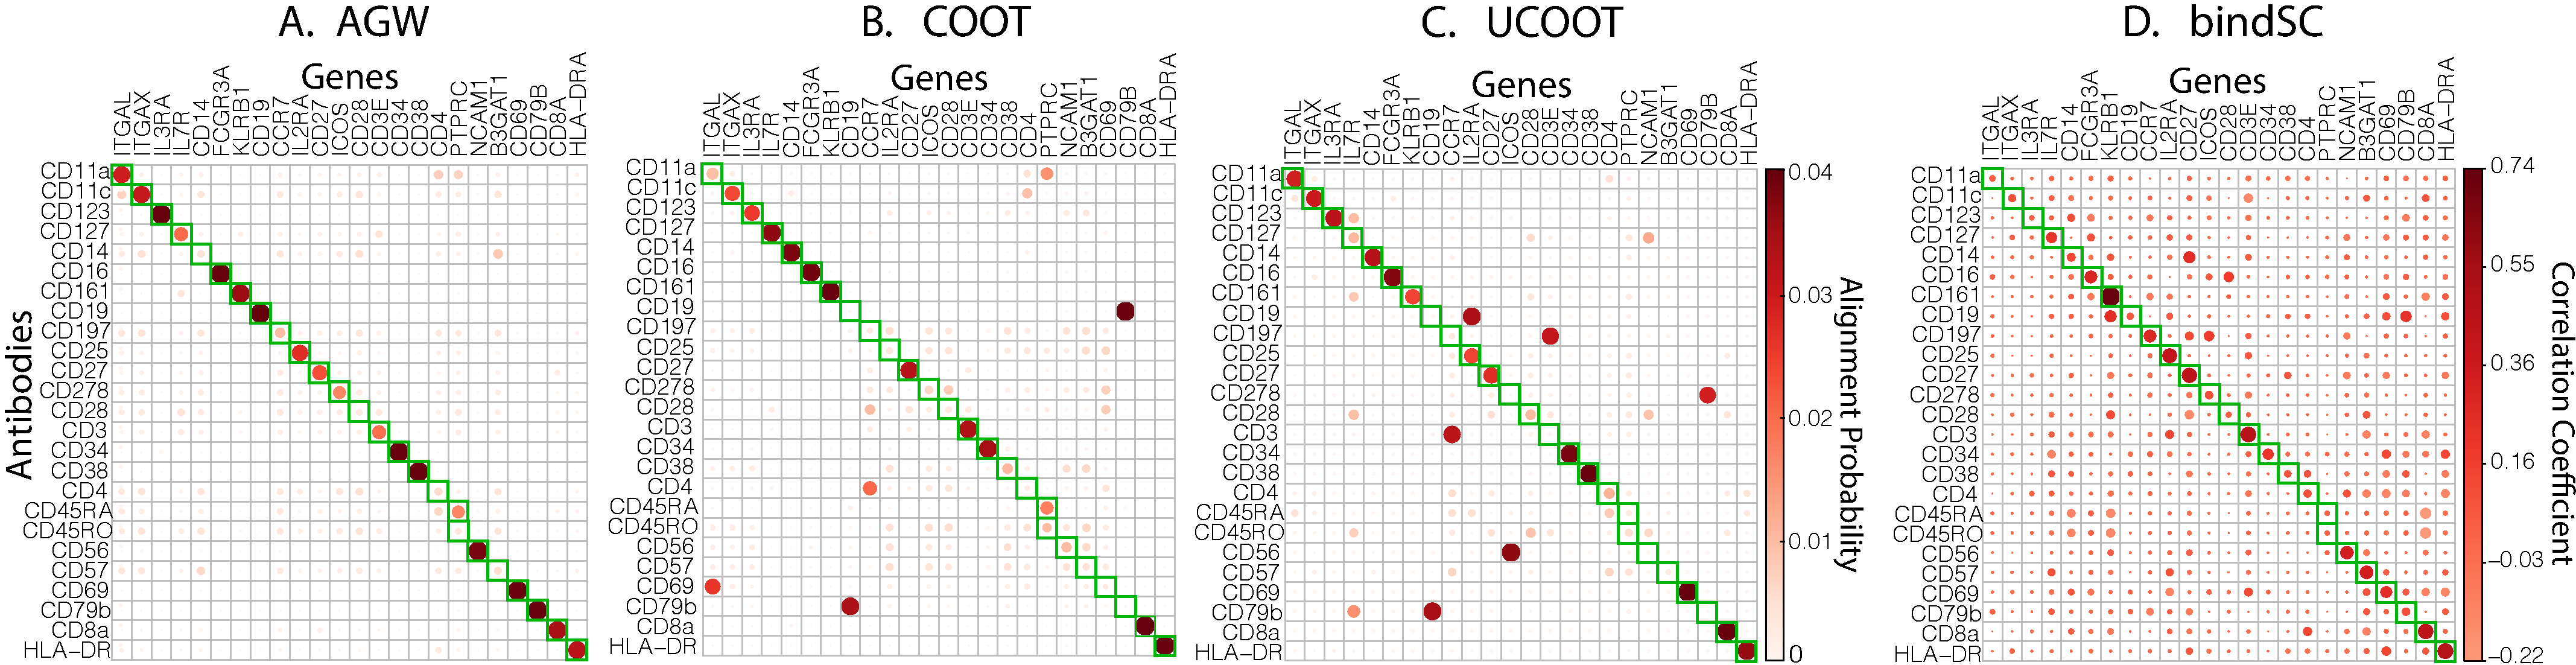
\includegraphics[width=\linewidth]{./Chapitre5/fig/cite_fgcoot_final.pdf}
\caption{\label{fig:cite} Feature alignments for the CITE-seq dataset. Green boxes indicate
where we expect matches (a notion of ``ground-truth'') based on domain knowledge.}
\end{figure}

\subsection{Integrating single-cell multi-omics datasets}
Integrating data from different single-cell sequencing experiments is
an important biological task for which OT has proven useful \citep{Pamona,UniPort,Demetci20}.
Single-cell experiments measure various genomic features at the individual cell resolution.
Jointly studying these can give scientists insight into the mechanisms regulating cells.
However, experimentally combining multiple types of measurements for the same cell
is challenging for most combinations. Scientists rely on the computational integration
of multi-modal data taken on different but related cells (\eg, by cell type or tissue)
to study the relationships and interactions between different aspects of the genome.

We particularly focus on this task for two reasons. First, GW is used as a state-of-the-art
method for this task \citep{Pamona,Demetci22,UniPort}, so it is important to see if
AGW improves upon it. Second, several single-cell benchmark datasets provide
ground-truth matchings on the feature- and the sample-level alignments.
This information allows us to assess the effect of guiding cross-domain matching with partial
or full prior knowledge of these relationships.

\paragraph{Single-cell alignment} We follow the first GW application in this domain
\citep{Demetci20} and align samples (\ie, cells) of simulated and real-world datasets
from different measurement types. We have ground-truth information on cell-cell alignments
for all datasets, which we only use for benchmarking. We demonstrate in \Cref{table:scCells}
that AGW consistently yields higher quality cell alignments (with lower alignment error)
compared to the state-of-the-art baselines, including GW, COOT, and their unbalanced counterparts.

We include bindSC as an additional baseline, which performs bi-order canonical correlation analysis
to align single-cell datasets. Unlike other single-cell alignment methods,
it internally computes a feature correlation matrix that users can extract. So,
we include it as a baseline to compare its feature alignment performance against
AGW in the next section. However, bindSC usage is limited to a few measurement types
as it requires an input matrix that relates features across domains to bring the datasets
into the same space at initialization. We do not have this information for most datasets,
thus the ``N/A'' entries in \Cref{table:scCells}.

% It is important to note that an unbalanced extension could be developed for AGW through future work to potentially further boost the results.

\paragraph{Aligning genomic features} AGW augments GW formulation with a feature coupling matrix.
Therefore, we jointly align features and see whether AGW reveals relevant biological relationships.
All current single-cell alignment methods only align samples (\ie, cells),
except for bindSC as discussed above.

Among the real-world datasets in \Cref{table:scCells}, CITE-seq \citep{CITEseq}
is the only one with ground-truth information on feature correspondences.
This dataset has paired single-cell measurements on the abundance levels of
25 antibodies and activity (i.e., ``expression'') levels of genes,
including the genes that encode these 25 antibodies. So, we first present
unsupervised feature alignment results on the CITE-seq dataset.
We compare our feature alignments with bindSC, COOT, and UCOOT in \Cref{fig:cite}.
The entries in the feature alignment matrices are arranged such that
the ``ground-truth'' correspondences lie in the diagonal, marked by green squares.
While AGW correctly assigns 19 out of 25 antibodies to their encoding genes with
the highest alignment probability, this number is 16 for UCOOT, 15 for COOT and
13 for bindSC (which yields correlation coefficients instead of alignment probabilities).
Additionally, the OT methods yield more sparse alignments thanks to
the ``least effort'' requirement in their formulation.

\begin{table}[t]
\begin{center}
\resizebox{1.0\linewidth}{!}{
\begin{tabular}{@{}lccccccccc@{}}
\toprule
               & \textbf{A $\rightarrow$ A} & \textbf{A $\rightarrow$ C} & \textbf{A $\rightarrow$ W} & \textbf{C $\rightarrow$ A} & \textbf{C $\rightarrow$ C} & \textbf{C $\rightarrow$ W} & \textbf{W $\rightarrow$ A} & \textbf{W $\rightarrow$ C} & \textbf{W $\rightarrow$ W} \\ \midrule


\textbf{AGW}   & \textbf{93.1$\pm$1.6}                               & \textbf{68.3$\pm$14.1}                              & \textbf{79.8$\pm$3.5}                               & \underline{55.4$\pm$7.1}                              & \underline{76.4$\pm$5.6}                               & \textbf{57.7$\pm$14.3}                              & 60.1$\pm$9.1                               & \textbf{60.9$\pm$13.3}                              & \textbf{97.3$\pm$0.9}                               \\
\textbf{GW}    & 86.2$\pm$2.3                               & 64.1$\pm$6.2                               & \underline{77.6$\pm$11.1}                              & 53.0$\pm$13.2                              & \textbf{81.9$\pm$10.5}                              & \underline{53.5$\pm$15.9}                              & 50.4$\pm$22.1                              & 54.3$\pm$14.7                              & 92.5$\pm$2.6                               \\
\textbf{COOT}  & 50.3$\pm$15.9                              & 35.0$\pm$6.4                               & 39.8$\pm$14.5                              & 40.8$\pm$15.8                              & 33.5$\pm$10.7                              & 37.5$\pm$10.4                              & 44.3$\pm$14.0                              & 27.4$\pm$10.2                              & 57.9$\pm$13.4                              \\
\textbf{UGW}   & \underline{90.6$\pm$6.5}                             & \underline{67.2$\pm$12.7}                            & 75.4$\pm$3.1                             & \textbf{56.3$\pm$14.6}                            & 69.2$\pm$8.7                            & 51.2$\pm$13.1                           & \textbf{66.7$\pm$9.9}                             & 58.4$\pm$4.7                            & \underline{94.7$\pm$1.5}                             \\
\textbf{UCOOT} & 65.4$\pm$2.1                              & 44.6$\pm$3.8                               & 36.4$\pm$1.2                               & 55.1$\pm$8.6                               & 52.1$\pm$3.8                               & 41.8$\pm$14.9                              & \underline{63.2$\pm$4.0}                               & \underline{59.7$\pm$6.3}                               & 80.3$\pm$2.1                               \\
\bottomrule
\end{tabular}}
\end{center}
\caption{\label{tab:hda_agw}
\textbf{Heterogeneous domain adaptation results (unsupervised)}.
Best results are bolded, and second-bests are underlined. For AGW,
the $\alpha$ values used are respectively $0.6, 0.9, 0.7, 0.9, 0.3, 0.8, 0.7, 0.2, 0.6$. }
\end{table}

\paragraph{Leveraging prior knowledge}
Finally, we show the advantage of providing priors by aligning a
multi-species gene expression dataset containing measurements from
the adult mouse prefrontal cortex \citep{mouse} and pallium of bearded lizard \citep{lizard}.
Since measurements come from two different species, the feature space (i.e., genes) differs,
and there is no 1-1 correspondence between the samples (i.e., cells). However,
there is a shared subset within the features, i.e., orthologous genes that
descend from a common ancestor and maintain similar biological functions in both species.
We also have domain knowledge on cells that belong to similar cell types across the two species.
Thus, we expect AGW to recover these relationships.

\begin{figure}[t]
\centering
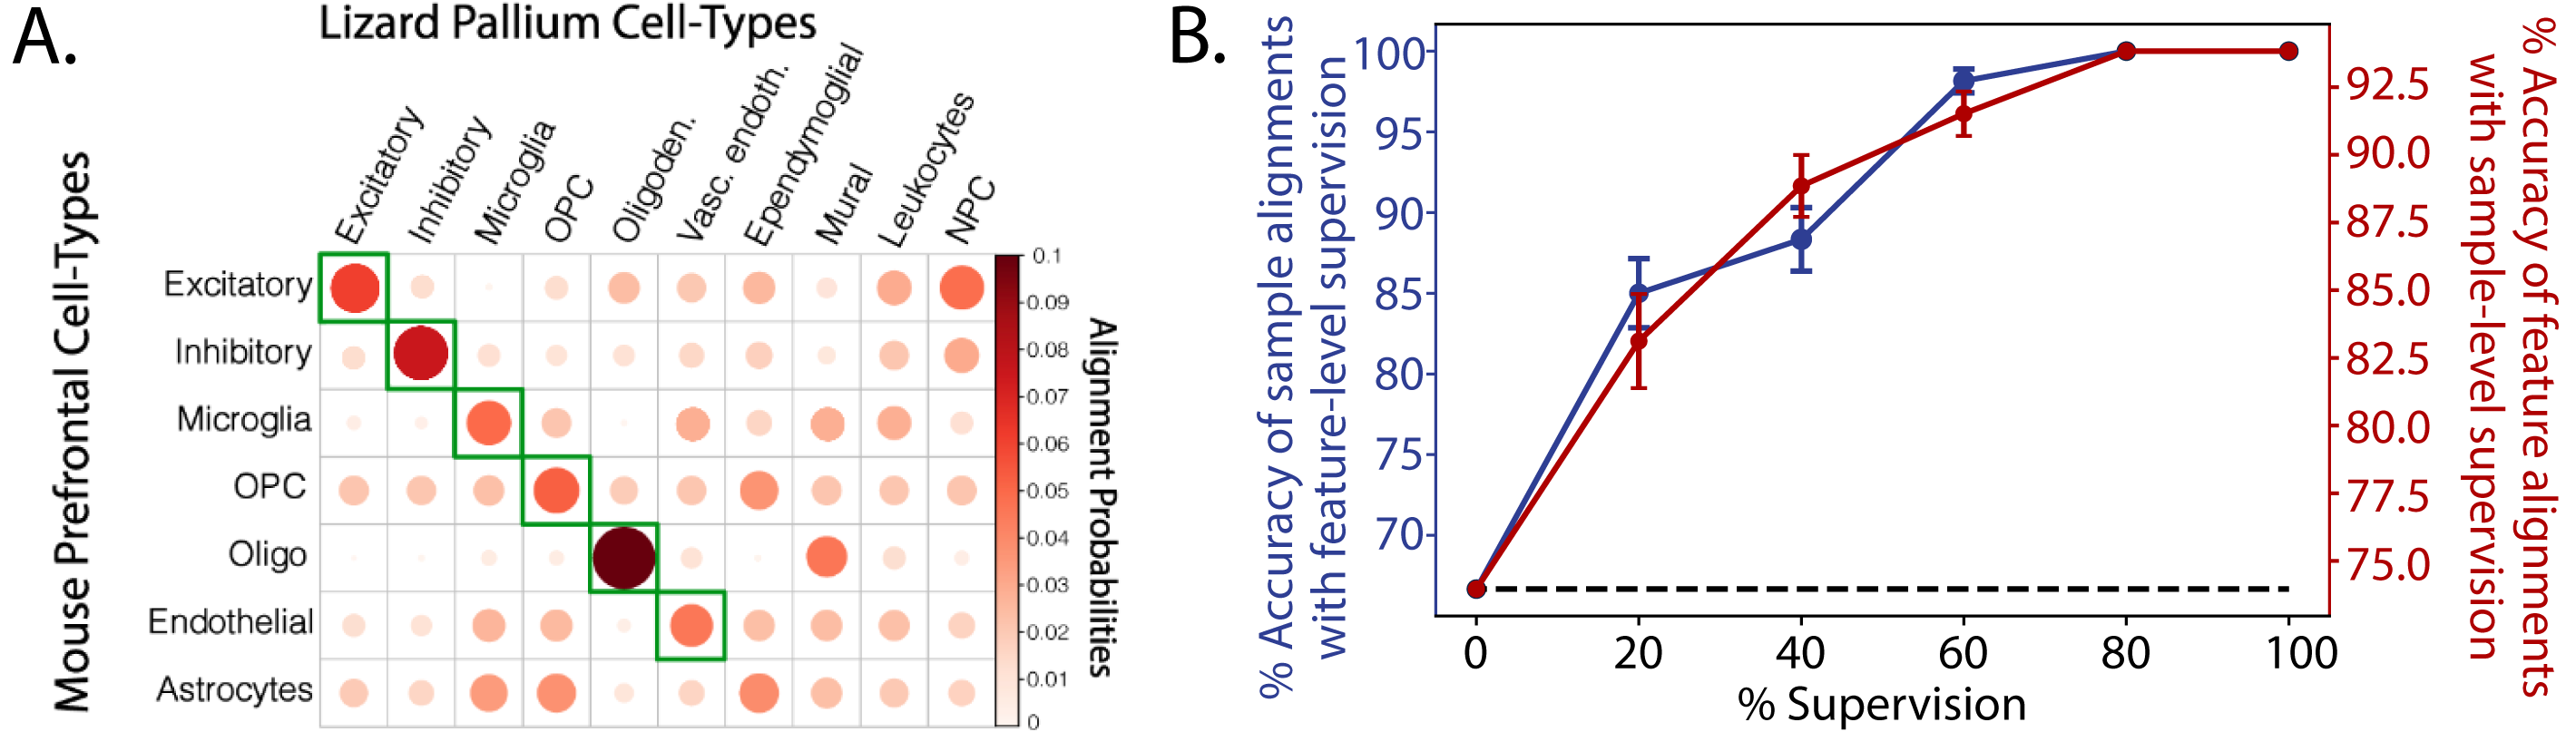
\includegraphics[width=\linewidth]{./Chapitre5/fig/xSp_full.png}
\caption{\label{fig:xsp} \textbf{Aligning cross-species dataset.}
A. AGW's cell-type alignments.
B. Providing supervision on one level of alignment (\eg, features)
boosts alignments on the other. Standard errors computed over 10 random runs.
Dashed line indicates the sample alignment performance of GW and bindSC
(orthologous gene used in input).}
\end{figure}

\Cref{fig:xsp}A visualizes the cell-type alignment probabilities yielded by AGW
when full supervision is provided on the $10,816$ orthologous genes.
The green boxes indicate alignment between similar types of cells.
This matrix is obtained by averaging the sample alignment matrix
(\ie, cell-cell alignments) into cell-type groups. We observe that
AGW yields biologically plausible alignments, as all the six cell types that
have a natural match across the two species are correctly matched.
We also show in \Cref{fig:xsp}B that providing supervision on one alignment level (\eg,
features) improves the quality on the other alignment level (\eg, samples).

%%%%%%%%%%%%%%%%%%%%%%%%%%%%%%%%%%%%%%%%%%%%%%
\subsection{Heterogeneous domain adaptation}

Finally, we demonstrate the generalizability of our approach on a popular ML task,
heterogeneous domain adaptation, where COOT and GW were previously successfully used.
Domain adaptation (DA) refers to the problem in which a classifier learned on one domain
(called \textit{source}) can generalize to the other (called \textit{target}). Here,
we apply AGW to unsupervised and semi-supervised heterogeneous DA (HDA) tasks,
where the source and target samples live in different spaces, and we have as few as
zero labeled target samples.

\paragraph{Datasets and experimental setup}
We follow the experimental setup by \citet{Redko20} and use source-target pairs
from the Caltech-Office dataset \citep{Saenko10}. We consider all pairs between three domains:
Amazon (A), Caltech-$256$ (C), and Webcam (W), whose images are embeddings from
the second last layer in the GoogleNet \citep{Szegedy15} (vectors in $\bbR^{4096}$)
and CaffeNet \citep{Jia14} (vectors in $\bbR^{1024}$) neural network architectures.

In semi-supervised settings, we incorporate prior knowledge on a few target labels
by adding an extra cost matrix to the training of sample coupling, so that
a source sample will be penalized if it transfers mass to the target samples from different classes.
Once the sample coupling $P$ is learned, we obtain the final prediction using label propagation:
$\widehat{y}_t = \argmax_k L_{k\cdot}$,
where $L = D_s P$ and $D_s$ denotes one-hot encodings of the source labels $y_s$.

All hyperparameters are tuned on a validation set based on accuracy.
We evaluate AGW against GW and COOT on source-target pairs from the Caltech-Office dataset
\citep{Saenko10} by considering all pairs between the three domains: Amazon (A), Caltech-$256$ (C),
and Webcam (W), similarly to \citep{Redko20}. We randomly choose 20 samples per class
and perform adaptation from CaffeNet to GoogleNet and repeat it 10 times.
We report the average performance of each method along with the standard deviation.
Differently than \citep{Redko20}, we (1) unit normalize the dataset prior to alignment
as we empirically found it to boost all methods' average performance compared to using
unnormalized datasets, (2) use cosine distances when defining intra-domain distance matrices
for GW and AGW, as we found them to perform better than Euclidean distances,
and (3) report results after hyperparameter tuning methods for each pair of datasets.
Specifically, for each pair of (A)-(C), (A)-(W), etc, we sweep a hyperparameter grid over
5 runs of random sampling, choose the best-performing combination, and run
10 runs of random sampling to report results.

For all methods that allow for entropic regularization,
we consider their version with no entropic regularization (either on the sample-level alignments,
feature-level alignments, or both), along with various levels of regularization.
For entropic regularization over sample alignments, we consider
$\varepsilon_1 \in [ 5e-4, 1e-3, 5e-3, 1e-2, 5e-2, 0.1] $. For entropic regularization over
feature alignments in COOT and AGW, we consider $\varepsilon_2 \in [ 5e-4, 1e-3, 5e-3, 1e-2, 5e-2, 0.1]$.
As the interpolation coefficient of AGW, we consider $\alpha \in [ 0.1, 0.2, ..., 0.9]$.

\paragraph{Results} \Cref{tab:hda_agw} presents the performance of each method averaged across
ten runs in the unsupervised setting, where AGW yields favorable results in 6 out of 9 cases.
In two cases, UGW, and in one case, UCOOT, outperform AGW despite the lower performance of
their balanced counterparts. In these cases, unbalanced formulations prove beneficial,
and support extending AGW to unbalanced scenarios as future work.

\section{Conclusion}

We present Augmented Gromov-Wasserstein (AGW), a new OT-based divergence for incomparable spaces.
It interpolates between GW and CO-Optimal transport and allows to narrow down the
choices of isometries induced by GW, while efficiently exploiting the prior knowledge
on the input data. We study its basic properties and empirically show that such restrictions
result in better performance for single-cell multi-omic alignment tasks and transfer learning.
Future work will focus on refining the theoretical analysis of the AGW invariants to
better understand their performance in practice. We will also extend AGW to the unbalanced
and/or continuous setting, and other tasks where feature supervision by domain experts
may be incorporated in OT framework.

\vfill